%
% CSE Electronic Homework Template
% Last modified 8/23/2018 by Jeremy Buhler

\documentclass[11pt]{article}
\usepackage[left=0.7in,right=0.7in,top=1in,bottom=0.7in]{geometry}
\usepackage{fancyhdr} % for header
\usepackage{graphicx} % for figures
\usepackage{amsmath}  % for extended math markup
\usepackage{amssymb}
\usepackage[bookmarks=false]{hyperref} % for URL embedding
\usepackage[noend]{algpseudocode} % for pseudocode
\usepackage[plain]{algorithm} % float environment for algorithms

%%%%%%%%%%%%%%%%%%%%%%%%%%%%%%%%%%%%%%%%%%%%%%%%%%%%%%%%%%%%%%%%%%%%%%
% STUDENT: modify the following fields to reflect your
% name/ID, the current homework, and the current problem number

% Example: 
%\newcommand{\StudentName}{Jeremy Buhler}
%\newcommand{\StudentID{123456}

\newcommand{\StudentName}{Dingyu Wang (Howard)}
\newcommand{\StudentID}{COMP 642: Machine Learning}
\newcommand{\HomeworkNumber}{2}

%%%%%%%%%%%%%%%%%%%%%%%%%%%%%%%%%%%%%%%%%%%%%%%%%%%%%%%%%%%%%%%%%%%%%%%%
% You can pretty much leave the stuff up to the next line of %%'s alone.

% create header and footer for every page
\pagestyle{fancy}
\fancyhf{}
\lhead{\textbf{\StudentName}}
\chead{\textbf{\StudentID}}
\rhead{\textbf{HW \HomeworkNumber}}
\cfoot{\thepage}

% preferred pseudocode style
\algrenewcommand{\algorithmicprocedure}{}
\algrenewcommand{\algorithmicthen}{}

% ``do { ... } while (cond)''
\algdef{SE}[DOWHILE]{Do}{doWhile}{\algorithmicdo}[1]{\algorithmicwhile\ #1}%

% ``for (x in y ... z)''
\newcommand{\ForRange}[3]{\For{#1 \textbf{in} #2 \ \ldots \ #3}}

% these are common math formatting commands that aren't defined by default
\newcommand{\union}{\cup}
\newcommand{\isect}{\cap}
\newcommand{\ceil}[1]{\ensuremath \left\lceil #1 \right\rceil}
\newcommand{\floor}[1]{\ensuremath \left\lfloor #1 \right\rfloor}

%%%%%%%%%%%%%%%%%%%%%%%%%%%%%%%%%%%%%%%%%%%%%%%%%%%%%%%%%%%%%%%%%%%%%%
\usepackage[utf8]{inputenc}
\usepackage[english]{babel}
\setlength{\parindent}{0em}
\setlength{\parskip}{1em}
 \usepackage{pythonhighlight}
\usepackage{graphicx}
\graphicspath{ {./images/} }


\begin{document}

% STUDENT: Your text goes here!

1) - 4) turned in in modules 2.1 and 2.2. \\ \\
5) \\
a) Red line on graph A.\\
b) Red line on graph B. \\
c) Circle on graph B. \\
d) Green line on graph B. \\
e) Removing the possible outliers would create a smaller mean squared error because the outlier points have a big effect on the (Predicted\_i - Actual\_i) terms.
\\
\\
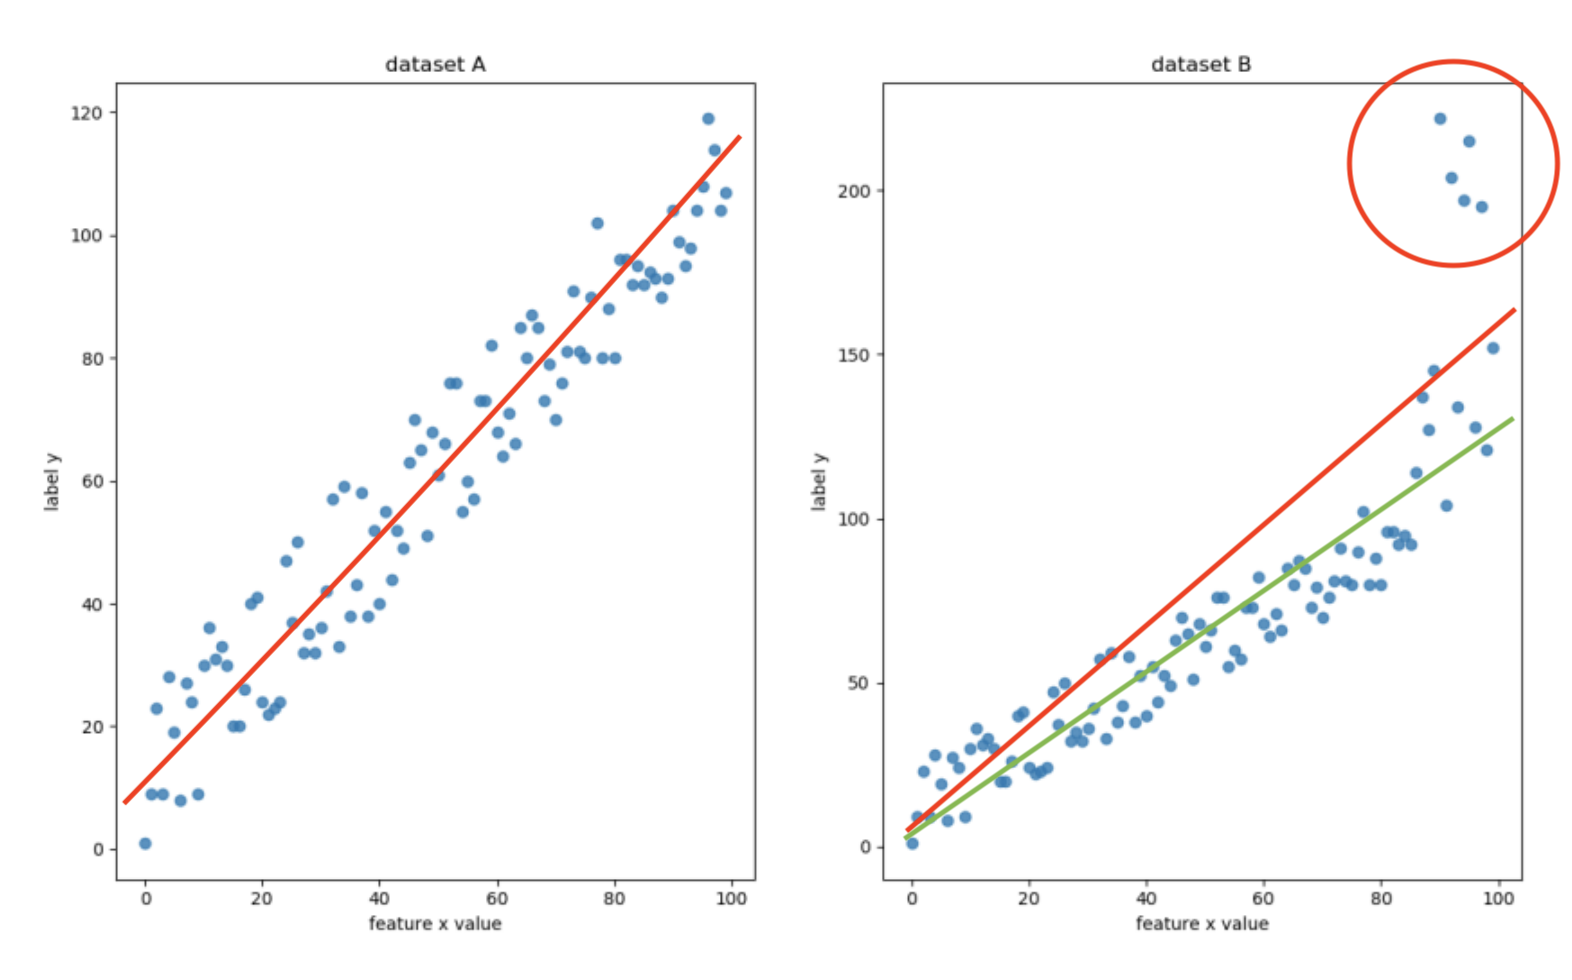
\includegraphics[scale=0.5]{pic1}
\\
\\
6) \\
a) Another way we can frame the problem is we want to predict the median house age in districts in California. This is a supervised learning problem since we have the response labels. This is a regression problem since response is numerical.\\

b) Based on the correlation matrix, we can conclude the coefficient sign for median\_income(B7), total\_rooms(B3), housing\_median\_age(B2), households(B6), total\_bedrooms(B4) are positive. These values in the correlation matrix are positive. We can conclude the coefficient sign for population(B5), longitude(B0), latitude(B1) are negative. These values in the correlation matrix are negative. The correlation matrix represents the magnitude of the relationship between variables, and that is similar to the interpretation of the coefficients.\\

c)  Looking at the describe function and plots, I decided to use 6 groups for housing\_median\_age. The data was spread between 0 - 50 years mostly, but has a spike at 51-53, so I included a 6th category. \\
\\
\\
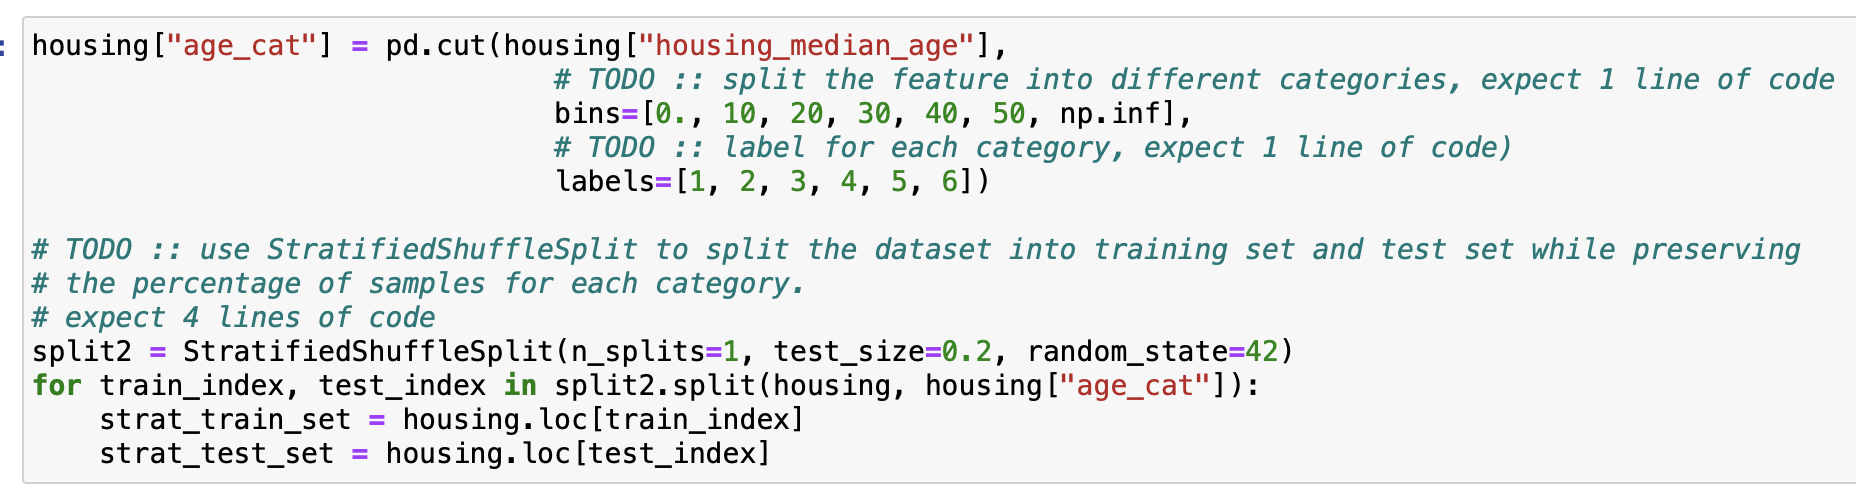
\includegraphics[scale=0.35]{pic2}
\\
\\
d) One hot encoding could be use when the category doesn't have a huge amount of different values and the data is not ordinal. Therefore, it could be used for a 'closest\_city' feature.\\

e) Having 0 error on the training data set probably means something went wrong or the model severely overfits the data. The error for test data would probably be very high for the model. It's usually always possible to increase model complexity to generate a lower error on the training data, but in machine learning, we care about how well the model predicts new data that it has not been seen.\\

f) \\
The best SVR predictor is linear and gets a RMSE of 105773.779.
kernel       rmse
linear: 105773.779
rbf: 117550.993
poly: 117330.949
sigmoid: 117101.023
precomputed: can't use, must be square

g) \\
GridSearchCV \\
final\_rmse: 49491.61792572629 
[47312.03285458, 51579.18220542] 

RandomizedSearchCV \\
final\_rmse: 50560.678 
[48372.88497456, 52657.65329852] 
\end{document}
